\chapter{Methods}

\section{The dendritic error model}

This section will go into detail about the dendritic error network \citep{sacramento2018dendritic}. The model contains a
somewhat complex and strongly recurrent connectivity, which poses one of the major criticisms aimed at it
\citep{whittington2019theories}. Much like traditional machine learning networks, it can be functionally separated into
layers. Yet in this particular model, input- hidden- and output layers are quite distinct in both neuron populations and
connectivity.


\subsection{Network architecture}

\begin{figure}[h!]
  \centering
  \begin{minipage}{0.5\textwidth}
    \centering
    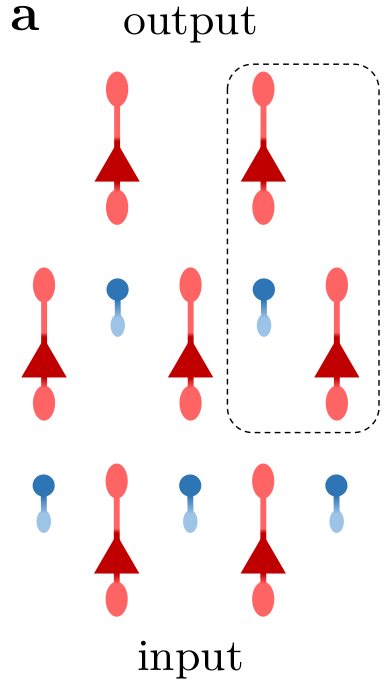
\includegraphics[width=0.9\textwidth]{network_a}
  \end{minipage}\hfill
  \begin{minipage}{0.4\textwidth}
    \centering
    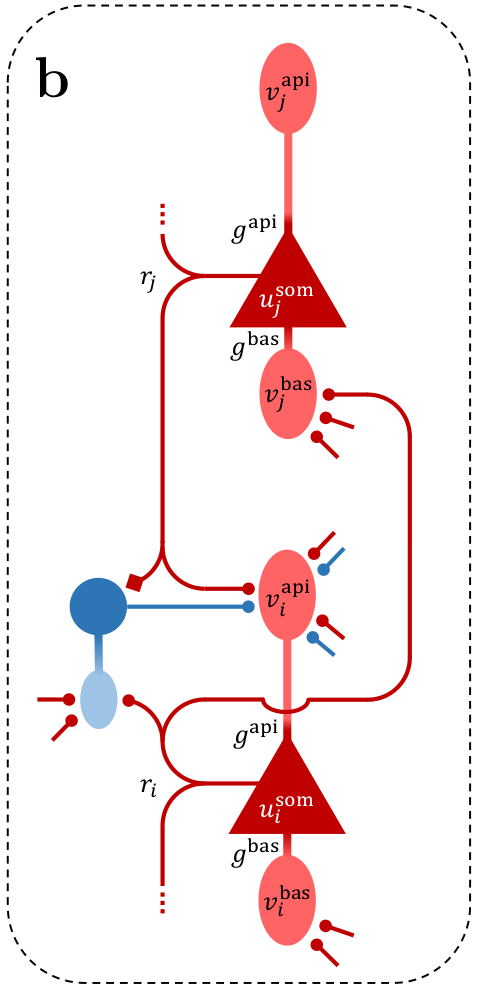
\includegraphics[width=0.9\textwidth]{network_b}
  \end{minipage}
  \caption[Structure of the dendritic error network]{Structure of the dendritic error network, from \citep{Haider2021}.
    \textbf{a:} pyramidal- (red) and interneurons (blue) in a network of three layers. Note the fact that the number
    interneurons in a layer is equal to the number of pyramidal neurons in the subsequent layer\protect\footnotemark.
    \textbf{b:} connectivity within the highlighted section. Feedback pyramidal-to-interneuron connections (displayed
    with rectangular synapse) transmit pyramidal somatic potential directly and connect to a single interneuron. This
    enables these interneurons to learn to match their corresponding next-layer pyramidal neurons. All other synapses
    (circles) transmit the neuron's somatic activation $\phi (u^{som})$ and fully connect their origin and target
    populations.}
  \label{fig-network}
\end{figure}

\footnotetext{{Note that the input layer is displayed as having interneurons here. This appears to be a mistake in the
      Figure. Within the implementation, interneurons are only modelled in hidden layers.}}

The basic connectivity scheme of the Model is shown in Fig. \ref{fig-network}. Neurons at the input layer receive no
feedback signals and serve primarily to apply a temporal low-pass filter to the stimulus which is injected directly into
their membrane.  Hidden layers consist of a pyramidal- and an interneuron population, which are fully connected to each
other reciprocally. Both types of neurons are represented by multi-compartment neuron models with leaky membrane
dynamics. Interneurons contain one somatic and one dendritic compartment, while pyramidal neurons are modeled with both
a basal and an apical dendrite.  Feedforward connections between layers are facilitated by all-to-all connections
between their respective pyramidal neurons and innervate basal compartments. Feedback connections from superficial
pyramidal neurons, as well as lateral interneuron connections arrive at the apical compartments of pyramidal neurons.
Thus, a hidden layer pyramidal neuron forms two reciprocal loops, one with all interneurons in the same layer, and one
with all pyramidal neurons in the next layer.

Interneurons receive feedback information from superficial pyramidal neurons in addition to their lateral connections.
These feedback connections are unique in this model, as they connect one pyramidal neuron to exactly one interneuron.
Instead of transmitting a neuronal activation as all other connections do, these connections relay somatic voltage
directly. This one-to-one connectivity puts a strict constraint on the number of interneurons in a hidden layer, as it
must be equal to the number of subsequent pyramidal neurons. These pairs of inter- and pyramidal neurons will henceforth
be called \textit{sister neurons}. The top-down signal serves to \textit{nudge} interneuron somatic activation towards
that of their pyramidal sisters. The purpose of an interneuron in this architecture is then, to predict the activity of
its sister neuron. Any failure to do so results in layer-specific errors which in turn are the driving force of learning
in this context, but more on this later.

Output layers have no interneurons, and are usually modeled as pyramidal neurons without an apical compartment. During
learning, the target for the network's activation is injected into their somatic compartment. Through the feedback
connections, it can propagate through the entire network. To understand what purpose this rather complex connectivity
scheme serves in our model, neuron models and plasticity rules require some elaboration.


\subsection{Neuron models}\label{sec-neurons}



The network contains two types of multi-compartment neurons; Pyramidal neurons with three compartments each, and
interneurons with two compartments each. They integrate synaptic inputs into dendritic potentials, which in turn leak
into the soma with specific conductances. Note that vector notation will be used throughout this section, and $u_l^P$
and $u_l^I$ denote the column vectors of pyramidal- and interneuron somatic voltages at layer $l$, respectively.
Synaptic weights $W$ are likewise assumed matrices of size $n \times m$, which are the number of output and input
neurons of the connected populations respectively. The activation (or rate) $r_l^P$ of pyramidal neurons is given by
applying the neuronal transfer function $\phi$ to their somatic potentials $u_l^P$:
\begin{align}
  r_l^P   & = \phi(u_l^P)                                                                      \\
  \phi(x) & = \begin{cases}
                0                                   & \textrm{if } \ x < -\epsilon               \\
                \gamma \ log(1+e^{\beta(x-\theta)}) & \textrm{if } \ -\epsilon \leq x < \epsilon \\
                \gamma \ x                          & \textrm{otherwise}
              \end{cases}
\end{align}

where $\phi$ acts component wise on $u$ and can be interpreted as a smoothed variant of ReLu (sometimes called
\textit{Softplus}) with scaling factors $\gamma=1$, $\beta=1$, $\theta=0$. Splitting the computation with the threshold
parameter $\epsilon=15$ does not alter its output much, but instead serves to prevent overflow errors for large absolute
values of $x$.

As mentioned before, pyramidal and interneurons are modeled as rate neurons with leaky membrane dynamics and multiple
compartments. Where applicable, they will be differentiated with superscripts $P$ and $I$ respectively. The basal and
apical dendrites of pyramidal neurons are denoted with superscripts $bas$ and $api$ respectively, while interneuron
dendrites are simply denoted $dend$.  The derivative somatic membrane potentials of layer $l$ pyramidal neurons is given
by:

\begin{align}
  C_m \dot{u}_l^P & = - g_l u_l^{P} + g^{bas} v_l^{bas} + g^{api} v_l^{api} \label{eq-pyr-dynamics-rate}
\end{align}

where $g_l$ is the somatic leakage conductance, and $C_m$ is the somatic membrane capacitance which will be assumed to
be $1$ from here on out. $v_l^{bas}$ and $v_l^{api}$ are the membrane potentials of basal and apical dendrites
respectively, and $g^{bas}$ and $g^{api}$ their corresponding coupling conductances.  Dendritic compartments in this
model have no persistence between simulation steps. Thus, they are defined at every timestep $t$ through incoming weight
matrices and presynaptic activities:

\begin{align}
  v_l^{bas}(t) & = W_l^{up} \ \phi(u_{l-1}^P(t)) \label{eq-v-bas-rate}                                     \\
  v_l^{api}(t) & =  W_l^{pi} \ \phi(u_l^I(t)) \ + \  W_l^{down} \ \phi(u_{l+1}^P(t)) \label{eq-v-api-rate}
\end{align}

The nomenclature for weight matrices conforms to \citep{Haider2021}, where they are indexed by the layer in which their
target neurons lie, and belong to one of four populations: Feedforward and feedback pyramidal-to-pyramidal connections
arriving at layer $l$ are denoted $W_l^{up}$ and $W_l^{down}$ respectively. Lateral pyramidal-to-interneuron connections
are denoted with $W_l^{ip}$ and their corresponding feedback connections with $W_l^{pi}$.

Interneurons integrate synaptic information by largely the same principle, but instead of top-down signals from their
sister neurons arriving at an apical compartment, it is injected directly into the soma.

\begin{align}
  C_m \dot{u}_l^I & = - g_l u_l^{I} + g^{dend} v_l^{dend} + i^{nudge, I}\label{eq-intn-dynamics} \\
  i^{nudge, I}    & = g^{nudge, I} u_{l+1}^P                                                     \\
  v_l^{dend}      & = W_l^{ip} \ \phi(u_{l}^P)
\end{align}

where $ g^{nudge, I}$ is the interneuron nudging conductance, and $u_{l+1}^P$ is the somatic voltage of pyramidal
neurons in the next layer.  Pyramidal neurons in the output layer $N$ effectively behave like interneurons, as they
receive no input to their apical compartment. Instead, the target  activation $u^{tgt}$ is injected into their soma:

\begin{align}
  C_m \dot{u}_N^P & = - g_l u_N^{P} + g^{bas} v_N^{bas} + i^{nudge, tgt} \\
  i^{nudge, tgt}  & = g^{nudge, tgt} u^{tgt}
\end{align}


These neuron dynamics correspond closely to those described in \citep{urbanczik2014learning}, including the extension to
more than two compartments which was proposed in the original paper. It should be noted however, that they are
simplified in some ways. These simplifications enabled the authors to prove analytically that this model approximates
Backprop. Yet they do come at the cost of omitting neuroscientific insights from the model, which will be discussed
later.

\section{Urbanczik-Senn Plasticity}\label{sec-urb-senn-plast}

The synapses in the network are all modulated according to variations of the "Urbanczik-Senn" plasticity rule
\citep{urbanczik2014learning}, which will be discussed in this section. Note that as for the neuron model, the dendritic
error model slightly simplifies some equations of the plasticity rule from its original implementation.

\subsection{Derivation}

The plasticity rule is defined for postsynaptic neurons which have one somatic and at least one dendritic compartment,
to the latter of which synapses of this type can connect. Functionally, synaptic weights are changed in such a way, as
to minimize discrepancies between the somatic activity and dendritic potential. This discrepancy is called the
\textit{dendritic prediction error}, and is computed from a hypothetical dendritic activation. The change in weight for
a synapse from neuron $j$ to the basal compartment of a pyramidal neuron $i$ is given by:

\begin{align}
  \dot{w}_{ij}    & = \eta \ ( \phi(u_i^{som}) - \phi(\hat{v}_i^{bas}) ) \ \phi(u_j^{som})^T \\
  \hat{v}_i^{bas} & = \alpha \  v_i^{bas}
\end{align}

with learning rate $\eta$, and $u^T$ denoting the transposition of the vector $u$ (which is by default assumed a column
vector). The dendritic prediction $\hat{v}_i^{bas}$ is a scaled version of the dendritic potential by the constant
factor $\alpha$, which is calculated from coupling and leakage conductances. As an example, basal dendrites of pyramidal
neurons in \citep{sacramento2018dendritic} are attenuated by $\alpha = \frac{g^{bas}}{g_l + g^{bas} + g^{api}}$. A key
property of this value for $\alpha$ is, that dendritic error is $0$ when the only input to a neuron stems from the given
dendrite. In other words, the dendrite predicts somatic activity perfectly, and no change in synaptic weights is
required. Neuron- and layer-specific differences in $\alpha$, as well as an analytical derivation are detailed in
\citep{sacramento2018dendritic}.

If a current is injected into the soma (or in this case, into a different dendrite), a dendritic error arises, and
plasticity drives synaptic weights to minimize it. In addition to the learning rate $\eta$, the change in weight
$\dot{w}_{ij}$ is proportional to presynaptic activity $\phi(u_j^{som})$. Therefore, a dendritic error arising without
presynaptic contribution does not elicit a change in that particular synapse. This ensures that only synapses are
modified which recently influenced the postsynaptic neuron, providing a form of credit assignment. Updates for the
weight matrices in a hidden layer $l$ of the dendritic error model are given by:

\begin{align}
  \dot{w}_{l}^{up}   & = \eta_l^{up} \ ( \phi(u_l^{P}) - \phi(\hat{v}_l^{bas}) ) \ \phi(u_{l-1}^{P})^T\label{eq-delta_w_up}         \\
  \dot{w}_{l}^{ip}   & = \eta_l^{ip} \ ( \phi(u_l^{I}) - \phi(\hat{v}_l^{dend}) ) \ \phi(u_{l}^{P})^T\label{eq-delta_w_ip}          \\
  \dot{w}_{l}^{pi}   & = \eta_l^{pi} \ - v_l^{api} \ \phi(u_l^{I})^T\label{eq-delta_w_pi}                                           \\
  \dot{w}_{l}^{down} & = \eta_l^{down} \ ( \phi(u_l^{P}) - \phi(w_l^{down} r_{l+1}^P) )\ \phi(u_{l+1}^{P})^T\label{eq-delta_w_down}
\end{align}

Each set of connections is updated with a specific learning rate $\eta$ and a specific dendritic error term. The purpose
of these particular dendritic errors will be explained in Section \ref{sec-selfpred}. Note that pyramidal-to-pyramidal
feedback weights $w_l^{down}$ are not plastic in the present simulations and are only listed for completeness, see
Section \ref{sec-feedback-plast} for more details on this case.

\section{The self-predicting network state}\label{sec-selfpred}

In the dendritic error model neuron dynamics, plasticity rules and network architecture form an elegant interplay, which
will be explained in this section. Since each interneuron receives a somatic nudging signal from its corresponding
sister neuron, incoming synapses from lateral pyramidal neurons adapt their weights to match feedforward
pyramidal-to-pyramidal weights. In intuitive terms; Feedforward pyramidal-to-pyramidal weights elicit a certain
activation in the subsequent layer, which is fed back into corresponding interneurons. Hence, in the absence of incoming
connections, nudging from sister neurons causes interneurons to take on a proportional somatic potential. In order to
minimize the dendritic error term in Equation \ref{eq-delta_w_ip}, pyramidal-to-interneuron weight matrices at every
layer must match these forward weights ($w_l^{ip} \approx \rho w_l^{up}$) up to some scaling factor $\rho$. The exact
value for $\rho$ is parameter-dependent and immaterial for now. As long as no feedback information arrives at the
pyramidal neurons, plasticity drives synaptic weight to fulfill this constraint. Note, that this alignment of two
separate sets of outgoing weights is achieved with only local information. Therefore, this mechanism could plausibly
align the weights of biological synapses that are physically separated by long distances. \newline

Next, consider the special case for interneuron-to-pyramidal weights in Equation \ref{eq-delta_w_pi}, in which
plasticity does not serve to reduce discrepancies between dendritic and somatic potential. The error term is instead
defined solely by the apical compartment voltage\footnote{In strict terms, it is defined by the deviation of the
dendritic potential from its specific reversal potential. Since that potential is zero throughout, $- v_l^{api}$ remains
as the error term.}. Thus, plasticity in these synapses works towards silencing the apical compartment. The apical
compartments also receive feedback from superficial pyramidal neurons, whose synapses will be considered non-plastic for
now. As shown above, interneurons each learn to match their respective sister neuron activity. Thus, silencing of apical
compartments can only be achieved by mirroring the pyramidal-to-pyramidal feedback weights ($w_l^{pi} \approx
  -w_l^{down}$).\newline

When enabling plasticity in only these two synapse types, the network converges on the "\textbf{self-predicting state}"
\citep{sacramento2018dendritic}. This state is defined by a minimization of four error metrics at each hidden layer $l$:

\begin{itemize}
  \item The symmetries between feedforward ($w_l^{ip} \approx \rho w_l^{up}$) and feedback ($w_l^{pi} \approx
          -w_l^{down}$) weights. \textit{Mean squared error (MSE)} between these pairs of matrices will be called
        \textbf{Feedforward - } and \textbf{Feedback weight error} respectively.
  \item Silencing of pyramidal neuron apical compartments ($v_l^{api} \approx 0$). Mean absolute apical compartment
        voltage within a layer is called the \textbf{Apical error}.
  \item Equal activations in interneurons and their respective sister neurons ($\phi (u_l^I) \approx \phi (u_{l+1}^P)$).
        The mean squared error over these vectors is called the \textbf{Interneuron error}.
\end{itemize}

The network does not ever reach a state in which all of these error terms are exactly zero. In the original
implementation, these deviations are minute and can likely be explained with floating point conversions. Since it is
impossible to replicate the timing of the original precisely within NEST, the NEST simulations deviate more strongly
from this ideal. The key insight here is that this state is not clearly defined by absolute error thresholds, but is
rather flexible. Thus, networks are able to learn successfully even when their weights are initialized imperfectly.


An analysis of the equations describing the network reveals that the idealized self-predicting state forms a stable
point of minimal energy. When Interneuron error is zero, the nudging signal from sister neurons is predicted perfectly,
thus disabling plasticity in incoming synapses. Likewise, a silenced apical compartment will disable plasticity in all
incoming synapses from interneurons. Furthermore, the apical compartment is also the driving factor for the dendritic
error of feedforward synapses (Equation \ref{eq-delta_w_up}), since any nonzero potential leaks into the
soma\footnote{This property might actually be considered the purpose of the Urbanczik-Senn plasticity. In the original
  paper, currents were injected directly into the soma to change the error term. In biological neurons, introducing a
  second dendrite which performs that very task makes far more sense.}. Thus, in the self-predicting state all plasticiy
in the network is disabled, and the state is stable regardless of the kind of stimulus injected into the input layer.
Next, notice how information flows backwards through the network; All feedback pathways between layers ultimately pass
through the apical compartments of pyramidal neurons. Thus, successful silencing of all apical compartments implies that
no information can travel backwards between layers. As a result, the network behaves strictly like a fully connected
feedforward network consisting only of pyramidal neurons. The recurrence within this network is in balance, and
completely cancels out its own effects. This holds true as long as the network only receives external stimulation at the
input layer. One interpretation of this is, that the network has learned to predict its own top-down input. A failure by
interneurons to fully explain (i.e. cancel out) top-down input thus results in a prediction error, encoded in deviation
of apical dendrite potentials from their resting state. This prediction error in turn elicits a cascade of plasticity in
several synapses, which drives the network towards a self-predicting state that is congruent with the novel top-down
signal. The authors show analytically that this intricate mechanism can be recast as a gradient descent optimization.



\section{Training the network}

Training the network then requires only the injection of a target activation into the network's output layer alongside
with a stimulus at the input layer. Since output layer neurons have strong feedback connections, a prediction error
arises in the previous layer. Synapses then drive to minimize this error by creating a new self-predicting state in
which interneurons mirror the novel behaviour of their sisters. Note that this interaction is not exclusive to the last
two layers. Any Apical errors elicit a change in somatic activity, which preceding interneurons will fail to predict.
Thus, errors are propagated backwards through arbitrarily deep networks, causing error minimization at every layer. See
the Supplementary analysis of \citep{sacramento2018dendritic} for a rigorous proof that this type of network does indeed
approximate the Backpropagation algorithm.



Classical Backprop relies on a strict separation of a forward pass of some stimulus, and subsequent a backwards pass
dependent on the arising loss at the output layer. Since the present network is time-continuous, stimulus and target
activation are injected into the network simultaneously. These injections are maintained for a given presentation time
$t_{pres}$, in order to allow the network to calculate errors through its recurrent connections before slowly adapting
weights. Particluarly for deep networks, signals travelling from both the input and output layer require some time to
balance out and elicit the correct dendritic error terms. This property poses the most significant drawback of this type
of time-continuous approximation of Backprop: The network tends to overshoot activations in some neurons, which in turn
causes an imbalance between dendritic and somatic compartments. This effect causes the network to change synaptic
weights away from the desired state during the first few milliseconds of a stimulus presentation. The solution
Sacramento et al. found for this issue was to drastically reduce learning rates, while increasing stimulus presentation
time. This solution is sufficient to prove that plasticity in this kind of network is able to perform error propagation,
but still has some issues. Most notably, training is highly inefficient and computationally intensive. A closer
investigation of the issue together with a different solution will be discussed in Section \ref{sec-latent-eq}.



\section{The NEST simulator}

One of the key research questions motivating this thesis is whether the network would be able to learn successfully when
employing spike-based communication instead of the rate neurons for which it was developed. As a framework for the
spike-based implementation two options were considered: The first one was to use the existing implementation of the
network which employs the Python frameworks \texttt{PyTorch} and \texttt{NumPy}, and expand it to employ spiking
neurons. PyTorch does in principle support spiking communication between layers, but is streamlined for implementing
less recurrent and less complex network and neuron models. Another concern is efficiency; PyTorch is very well optimized
for computing matrix operations on dedicated hardware. This makes it a good choice for simulating large networks of rate
neurons, which transmit all of their activations between layers at every simulation step. Spiking communication between
leaky neurons is almost antithetical to this design philosophy and thus can be expected to perform comparatively poorly
when using this backend.

The second option was to use the NEST simulator
(\href{https://nest-simulator.readthedocs.io}{nest-simulator.readthedocs.io}, \cite{Gewaltig2007}), which was developed
with highly parallel simulations of large spiking neural networks in mind. It is written in C++ and uses the
\textit{Message Passing Interface} (\href{https://www.mpi-forum.org/}{MPI}) to efficiently communicate events between
both threads and compute nodes. One design pillar of the simulator, which is particularly relevant for this project, is
the event-based communication scheme that underpins all simulated nodes. It ensures that communication bandwidth at
every simulation step is only used by the subset of nodes which transmit signals at that time step, which is
particularly efficient for spiking communication. Another important advantage of the NEST simulator is, that an
event-based implementation of the Urbanczik-Senn plasticity alongside a corresponding neuron model had already been
developed for it. Therefore, it was decided to implement the spiking neuron model in the NEST simulator.

The simulator has one particular limitation which needs to be considered. As communication between physically separate
compute nodes takes time, Events\footnote{An Event in NEST is an abstract C++ Class that is created by neurons, and
  transmitted across threads and compute nodes by the Simulator. A Multitude of Event types are provided (i.e.\
  \texttt{SpikeEvent, CurrentEvent, RateEvent}), each able to carry specific types of payload and being processed
  differently by postsynaptic neurons.} in NEST can not be handled in the same simulation step in which they were sent.
Thus, NEST enforces a synaptic transmission delay of at least one simulation step for all connections. This property is
integral to other parallel simulation backends \citep{Hines1997} as well as neuromorphic hardware
\citep{davies2018loihi}. It may not even considered a limitation by some, as synaptic transmission within biological
neurons is never instantaneous either \citep{kandel2021principles}. Yet particularly with regard to the relaxation
period issue of this model (cf. Section \ref{sec-latent-eq}), it can be expected to affect performance.


\section{Transitioning to spiking communication}

The spiking neuron models rely heavily on the NEST implementation from Stapmanns and colleagues \citep{Stapmanns2021},
which was used show that spiking neurons are able to perform learning tasks that were designed for the rate neurons
described in \citep{urbanczik2014learning}. The existing model is an exact replication of the Urbanczik-Senn neuron in
terms of membrane dynamics. The critical update of the NEST variant is that instead of transmitting their hypothetical
rate $r = \phi(u)$ at every time step, these neurons emit spikes in a similar way to stochastic binary neurons
\citep{Ginzburg1994}. The number of spikes to be generated during a simulation step $n$ is determined by drawing from a
Poisson distribution, which takes $r$ as a parameter:

\begin{align}
  P\{\textit{n} \ \text{spikes during} \ \Delta t\} & = e^{-r \Delta t} \frac{(r \ \Delta t) ^ n}{n!}\label{eq-pr-n-spikes} \\
  \langle \textit{n} \rangle                        & = r \ \Delta t \label{eq-n-spikes}
\end{align}

where $\Delta t$ denotes the integration time step of the simulator, which will be assumed to be $0.1 ms$ from here on
out.  $\langle \textit{n} \rangle$ denotes the expected number of spikes to be emitted in a simulation step. Note that
this mechanism makes the assumption that more than one spike can occur per simulation step. NEST was developed with this
possibility in mind and provides a \textit{multiplicity} parameter for SpikeEvents, which is processed at the
postsynaptic neuron. As the high spike frequencies resulting from this could not occur in biological neurons, the model
is also capable of simulating a refractory period. For this, the number of spikes per step is limited to $1$, and the
spiking probability is set to 0 for the duration of the refractory period $t_{ref}$. The probability of at least one
spike occurring within the next simulation step is given the inverse probability of no spike occurring. Thus, when
inserting $n=0$ into Equation \ref{eq-pr-n-spikes}, the probability of eliciting at least one spike within the next
simulation step can be derived as:

\begin{align}
  P\{ \textit{n} \geq 1\} & = 1 - e^{-r \Delta t}
\end{align}


Drawing from this probability then determines whether a spike is sent during that step, henceforth denoted with the
function $s(t)$, which outputs $1$ if a spike is sent during the interval $[t, t+\Delta t]$, and $0$ otherwise.
\newline

In order to implement the plasticity rule for spiking neurons, dendritic compartments need to be modeled with leaky
dynamics. These dynamics are fundamentally the same as those described for the somatic compartment. Thus, the basal
compartment of a pyramidal neuron $j$ evolves according to:

\begin{align}
  C_m^{bas} \dot{v}_j^{bas} & = -g_l^{bas} \  v_j^{bas} + \sum_{i \in I} W_{ji} s_i(t)     \label{eq-spiking-basal-compartment}
\end{align}

with presynaptic neurons $I$, and membrane capacitance $C_m^{bas}$ and leakage conductance $g_l^{bas}$ being specific to
the basal dendrite. Note that these equations are calculated individually for each neuron and do not employ the matrix
notation used for layers of rate neurons. Pyramidal apical and interneuron dendritic compartments evolve by the same
principle and with largely the same parameters.

\section{Event-based Urbanczik-Senn plasticity}\label{sec-event-urb}

One major challenge in implementing this architecture with spiking neurons is the Urbanczik-Senn plasticity introduced
in Section \ref{sec-urb-senn-plast}. Since the plasticity rule is originally defined for rate neurons, computing the
updates for spiking neurons requires some additional effort. Fortunately, this problem has already been solved in NEST
for two-compartment neurons \citep{Stapmanns2021}. This Section will discuss its algorithm and its implementation.
\newline

Since NEST is an event-based simulator, most of the plasticity mechanisms developed for it compute weight changes at the
location (i.e. thread and compute node) of the postsynaptic neuron whenever an Event is received. This has several
advantages; It allows the thread that created the Event to continue processing neuron updates instead of having to
synchronize with all threads that manage recipient neurons.  More importantly, this feature mirrors the local properties
of most biologically plausible synaptic plasticity models, as these are often considered to be primarily dependent on
factors that are local to the synapse \citep{magee2020synaptic}. For a spiking implementation of the Urbanczik-Senn
plasticity, dendritic errors at every time step are required instead of just a scalar trace at the time of a spike, as
would be the case for STDP. Thus, a mechanism for managing these errors was required, for which two basic possibilities
were considered:

In a \textbf{Time-driven scheme}, dendritic errors are made available to synapses at every timestep, and weight changes
are applied instantaneously. This approach is in principle an adaptation of the original computations for spiketrains.
Its main drawback is that calls to the synaptic update function are as frequent as neuron updates - for all synapses.
Particularly for large numbers of incoming synapses, as is common for simulations of cortical pyramidal neurons
\citep{potjans2014cell,vezoli2004quantitative}, this requires numerous function calls per time step.  Therefore, this
approach proved costly in terms of computational resources.

An \textbf{Event-driven scheme} on the other hand, updates synaptic weights only when a spike is sent through the
synapse. A history of the dendritic error is stored at the postsynaptic neuron, which is read by each synapse when a
spike is transmitted in order to compute weight changes. As the history of dendritic error applies equally to all
incoming synapses, it only needs to be recorded once at the neuron. Alongside each entry in the history, a counter is
stored and incremented whenever a synapse has read the history at that time step. Once all synapses have read out an
entry, it is deleted. Thus, the history dynamically grows and shrinks during simulation and is only ever as long as the
largest inter-spike interval (ISI) of all presynaptic neurons. This approach proves to be more efficient in terms of
computation time, since fewer calls to the update function are required per synapse. It does come at the cost of memory
consumption, as the history can grow particularly large for simulations with low in-degrees or large ISI\footnote{It
  should also be noted that in this approach requires redundant integration of the history by every synapse. Stapmanns et
  al. propose a third solution, in which this integration is performed once whenever a spike is transmitted through any
  incoming connection, with the resulting weight change being applied to all synapses immediately. This approach proved to
  be even more efficient for some network configurations, but is incompatible with simulations where incoming synapses
  have heterogeneous synaptic delays due to the way that these delays are processed by the NEST simulator. See Section
  3.1.3 in \citep{Stapmanns2021} for a detailed explanation.}. During testing, the Event-based schemed proved
substantially more efficient for many network types. This did however introduce the challenge of retroactively computing
weight changes from the time of the last spike upon arrival of a new spike. \newline


\subsection{Integrating weight changes}


Stapmanns et al. describe the Urbanczik-Senn plasticity rule based on the general equation for weight changes, while
omitting obsolete parameters:

\begin{align}
  \dot{w}_{ij}(t) & = F(s_j^\ast (t), V_i^\ast (t)) \label{eq-delta-w-spiking}
\end{align}

where the change in weight $\dot{w}_{ij}$ of a synapse from neuron $j$ to neuron $i$ at time $t$ is given by a function
$F$ that depends on the postsynaptic membrane potential $V_i^\ast$ and the presynaptic spiketrain $s_j^\ast$. The $\ast$
operator denotes a causal function, indicating that a value $V_i^\ast(t)$ potentially depends on all previous values of
$V_i(t' < t)$. One can formally integrate Equation \ref{eq-delta-w-spiking} in order to obtain the weight change between
two arbitrary time points $t$ and $T$:

\begin{align}
  \Delta w_{ij}(t,T) & = \int_t^T dt' F[s_j^\ast, V_i^\ast](t') \label{eq-delta-w-t-T}
\end{align}

This integral forms the basis of computing the change in weight between two arriving spikes. Thus, at the
implementational level, $t$ is usually the time of the last spike that traversed the synapse, and $T$ is the current
\texttt{biological\_time}\footnote{This term is adopted from the NEST convention, where it describes the time in $ms$
  which the simulator has computed. In other words, it is the number of simulation steps times $\Delta t$, not to be
  confused with a simulation's hardware-dependent runtime (sometimes also called \textit{wall clock time}
  \citep{albada2018performance}). }. For spiking neurons, it is necessary to approximate the presynaptic rate
($r_j=\phi(u_j)$). For this, a well established solution is to transform the spiketrain $s_j$ into a decaying trace
using an exponential filter kernel $\kappa$:

\begin{align}
  \kappa(t)     & = H(t) \frac{1}{t}e^{\frac{-t}{\tau_{\kappa}}}                        \\
  H(t)          & =
  \begin{cases}
    1 & \text{if $t > 0$}    \\
    0 & \text{if $t \leq 0$} \\
  \end{cases}                                                              \\
  (f \ast g)(t) & = \int_{- \infty }^{\infty} f(t') g(t-t') d t' \label{eq-convolution} \\
  s_j^\ast      & = \kappa_s \ast s_j. \label{eq-spike-trace}
\end{align}

with filter time constant $\tau_\kappa$. The trace is computed by convolving (Equation \ref{eq-convolution}) the
spiketrain with the exponential filter kernel $\kappa$. The filter uses the Heaviside step function $H(t)$, and is
therefore only supported on positive values of $t$ (also called a one-sided exponential decay kernel). This property is
important, as integration limits of the convolution can be truncated when $f$ and $g$ are both only supported on
$[0,\infty)$:

\begin{align}
  (f \ast g)(t) & = \int_{0}^{t} f(t') g(t-t') d t'
\end{align}

Since spikes naturally only occur for $t>0$, this simplified integral allows for a much more efficient computation of
the convolution. The Function $F$ on the right-hand side of Equation \ref{eq-delta-w-spiking} can therefore be rewriten
as:

\begin{align}
  F[s_j^\ast, V_i^\ast] & = \eta \kappa \ast (V_i^\ast s_j^\ast)        \\
  V_i^\ast              & = (\phi(u_i^{som}) - \phi(\hat{v}_i^{dend}) )
\end{align}

with learning rate $\eta$. $V_i^\ast$ then is the dendritic error of the dendrite that the
synapse between $j$ and $i$ is located at\footnote{The dendritic error here is defined as the difference between two
hypothetical rates based on the arbitrary function $\phi$. The original implementation uses the difference between the
true postsynaptic spiketrain and this dendritic prediction ($V_i^\ast = (s_i - \phi(\hat{v}_i^{dend}) )$).
Furthermore, Stapmanns et al. show that generating a spiketrain from the dendritic potential ($V_i^\ast = (s_i -
  s_i^{dend})$) also results in successful learning, although at the cost of additional training time. The rate-based
variant was chosen in order to not hinder learning performance any more than necessary.}. Writing out the convolutions
in Equation \ref{eq-delta-w-t-T} explicitly, we obtain

\begin{align}
  \Delta w_{ij}(t,T) & = \int_t^T dt' F[s_j^\ast, V_i^\ast](t')                                                                           \\
                     & =  \int_t^T dt' \  \eta\int_0^{t'} dt'' \ \kappa(t'-t'') V_i^\ast (t'') s_j^\ast (t'') \label{eq-delta-w-t-T-long}
\end{align}

Computing this Equation directly is somewhat inefficient due to the nested integrals. Yet, the authors show that it is
possible to break up the integrals into two simpler computations and rewrite the weight change as:


\begin{align}
  \Delta W_{ij}(t, T) & = \eta \left[ I_1 (t, T) - I_2(t,T) + I_2(0,t)\left( 1- e^{-\frac{T-t}{\tau_\kappa}} \right) \right]\label{eq-proof-start} \\
  I_1(a, b)           & = -\int_{a}^{b} dt \ V_i^\ast (t) s_j^\ast (t)                                                                             \\
  I_2(a, b)           & = -\int_{a}^{b} dt \ e^{-\frac{b-t}{\tau_\kappa}} V_i^\ast (t) s_j^\ast (t)\label{eq-proof-end}                            \\
\end{align}

See Section 5.1 in \citep{Stapmanns2021} for a rigorous proof that this is in fact the desired integral. The resulting
equations allow for a rather efficient computation of weight changes compared to the complex integral described in
Equation \ref{eq-delta-w-t-T-long}. This integration is performed whenever a spike traverses a synapse. It generalizes
to all special cases in Equations \ref{eq-delta_w_up}-\ref{eq-delta_w_down}, as long as the appropriate dendritic
error is stored by the postsynaptic neuron.

\section{Latent Equilibrium}\label{sec-latent-eq}

The most significant drawback of the Sacramento model is the previously mentioned requirement for long stimulus
presentation times and appropriately low learning rates. This makes the network prohibitively inefficient for the large
networks required for complex learning tasks. Sacramento et al. developed a steady-state approximation of their network
which models the state of the network after it has balanced out in response to a stimulus-target pair. It does not
suffer from these issues and shows that their model can in principle solve more demanding learning tasks such as MNIST.
Yet these types of approximation are much further detached from biological neurons than the original model and thus do
not lend themselves well to an investigation of biological plausibility \citep{Gerstner2009}. Furthermore, the
approximation is unsuitable for and investigation of spike-based communication, since the steady state of both network
ideally would be the same. Thus, neither the fully modeled neuron dynamics nor the steady-state approximation are suited
for complex learning tasks. A substantial improvement to rate neurons which promises to solve this dilemma was developed
by \citep{Haider2021}, and will be discussed here.
\newline

The requirement for long stimulus presentation times of the dendritic error network is caused by the slow development of
leaky neuron dynamics, and is therefore not unique to this model. When a stimulus-target pair is presented to the
network, membrane potentials in all neurons slowly evolve until a steady state is reached. The time until a network of
has reached this state after a change in input is called the \textit{relaxation period} following \citep{Haider2021}.
Given a membrane time constant $\tau_m$, a feedforward network with $N$ layers of leaky neurons thus has a relaxation
time constant of $N \tau_m$. Yet in our case, a target activation simultaneously injected into the output neurons slowly
propagates backwards through the highly recurrent network. Neurons at early layers require all subsequent layers to be
fully relaxed in order to correctly compute their dendritic error terms, effectively being dependent on two network
passes. Haider et al. state that this kind of network therefore requires $2N\tau_m$ to relax in response to a given
input-output pairing. This prediction proved to be slightly optimistic in experiments, as shown in Fig.
\ref{fig-error-comp-le}.

This is a major issue, as it implies that plasticity during the first few miliseconds of a stimulus presentation is
driven by faulty error terms. The network thus tends to 'overshoot', and needs to undo the synaptic weight changes made
during the relaxation period in the later phase of a stimulus presentation, in order to make tangible progress on the
learning task. Haider et al. call this issue the "relaxation problem" and suggest that it might be inherent to most
established attempts at biologically plausible Backpropagation algorithms
\citep{Whittington2017,guerguiev2017towards,sacramento2018dendritic,millidge2020activation}.



The choice to simply increase presentation time to compensate for the relaxation period is therefore somewhat
problematic. It implicitly tolerates adverse synaptic plasticity in all synapses, which are counteracted by enforcing
the desired plasticity for a longer time. Physiological changes that are meant to immediately be undone are of course an
inefficient use of a brain's resources, which can be considered highly untypical for a biological system. One possible
solution to this is to decrease synaptic time constants and remove the temporal filtering of stimulus injections. Yet
this does not solve the fundamental issue that during a substantial portion of stimulus presentations, the network is
driven by erroneous plasticity. Removing temporal filtering does decrease the length of the relaxation period, but
causes a drastic increase in dendritic error values during that period. Therefore, while improving response time, this
change effectively impedes learning. Another possible solution is to disable plasticity for the first few milliseconds
of stimulus presentation. After the network has relaxed, the plasticity rules produce useful weight changes and learning
rates can consequently be safely increased. Yet a mechanism by which neurons could implement this style of phased
plasticity is yet to be found, making this approach questionable in terms of biological plausibility. Furthermore, it
introduces a requirement for external control to the network, a trait that is considered highly undesirable for
approximations of Backprop \citep{whittington2019theories}. Ideally, the relaxation period would be skipped or
shortened, in order to reduce the erroneous plasticity. This would allow for a loosening of the constraints put on
presentation time and learning rates, thus increasing computational efficiency. \newline



The approach proposed by Haider et al. is to change the parameter of the activation function $\phi$, a mechanism called
\textit{Latent Equilibrium} (LE). Neurons in the original dendritic error network (henceforth called \textit{Sacramento
  neurons}) transmit a function of their somatic potential $u_i$, which is updated through Euler integration at every
simulation step (Equation \ref{eq-r-t-sacramento}). In contrast, neurons using Latent Equilibrium (henceforth called
\textit{LE neurons}) transmit a function of what the somatic potential is expected to be in the future. To calculate
this expected future somatic potential $\breve{u}$, the integration is performed with a larger Euler step:

\begin{align}
  u_i(t+ \Delta t)          & = u_i(t) + \dot{u}_i(t) \ \Delta t \label{eq-r-t-sacramento} \\
  \breve{u}_i(t + \Delta t) & = u_i(t) + \dot{u}_i(t) \ \tau_{eff} \label{eq-r-t-haider}
\end{align}

Instead of broadcasting their rate based on the current somatic potential ($r_i(t) = \phi(u_i(t))$), LE neurons send
their predicted future activation, denoted as $\breve{r}_i(t) = \phi(\breve{u}_i(t))$. The degree to wich LE neurons
look ahead is determined by the \textit{effective membrane time constant} $\tau_{eff} = \frac{C_m}{g_l + g^{bas} +
    g^{api}}$. This time constant takes into account the conductance with which dendritic compartments leak into the soma,
which is a key driving factor for the speed at which the network relaxes. Any computations that employ or relate to this
prediction of future network states will henceforth be referred to as \textit{prospective} and denoted with a breve
($\breve{x}$).


\begin{figure}[h!]
  \centering
  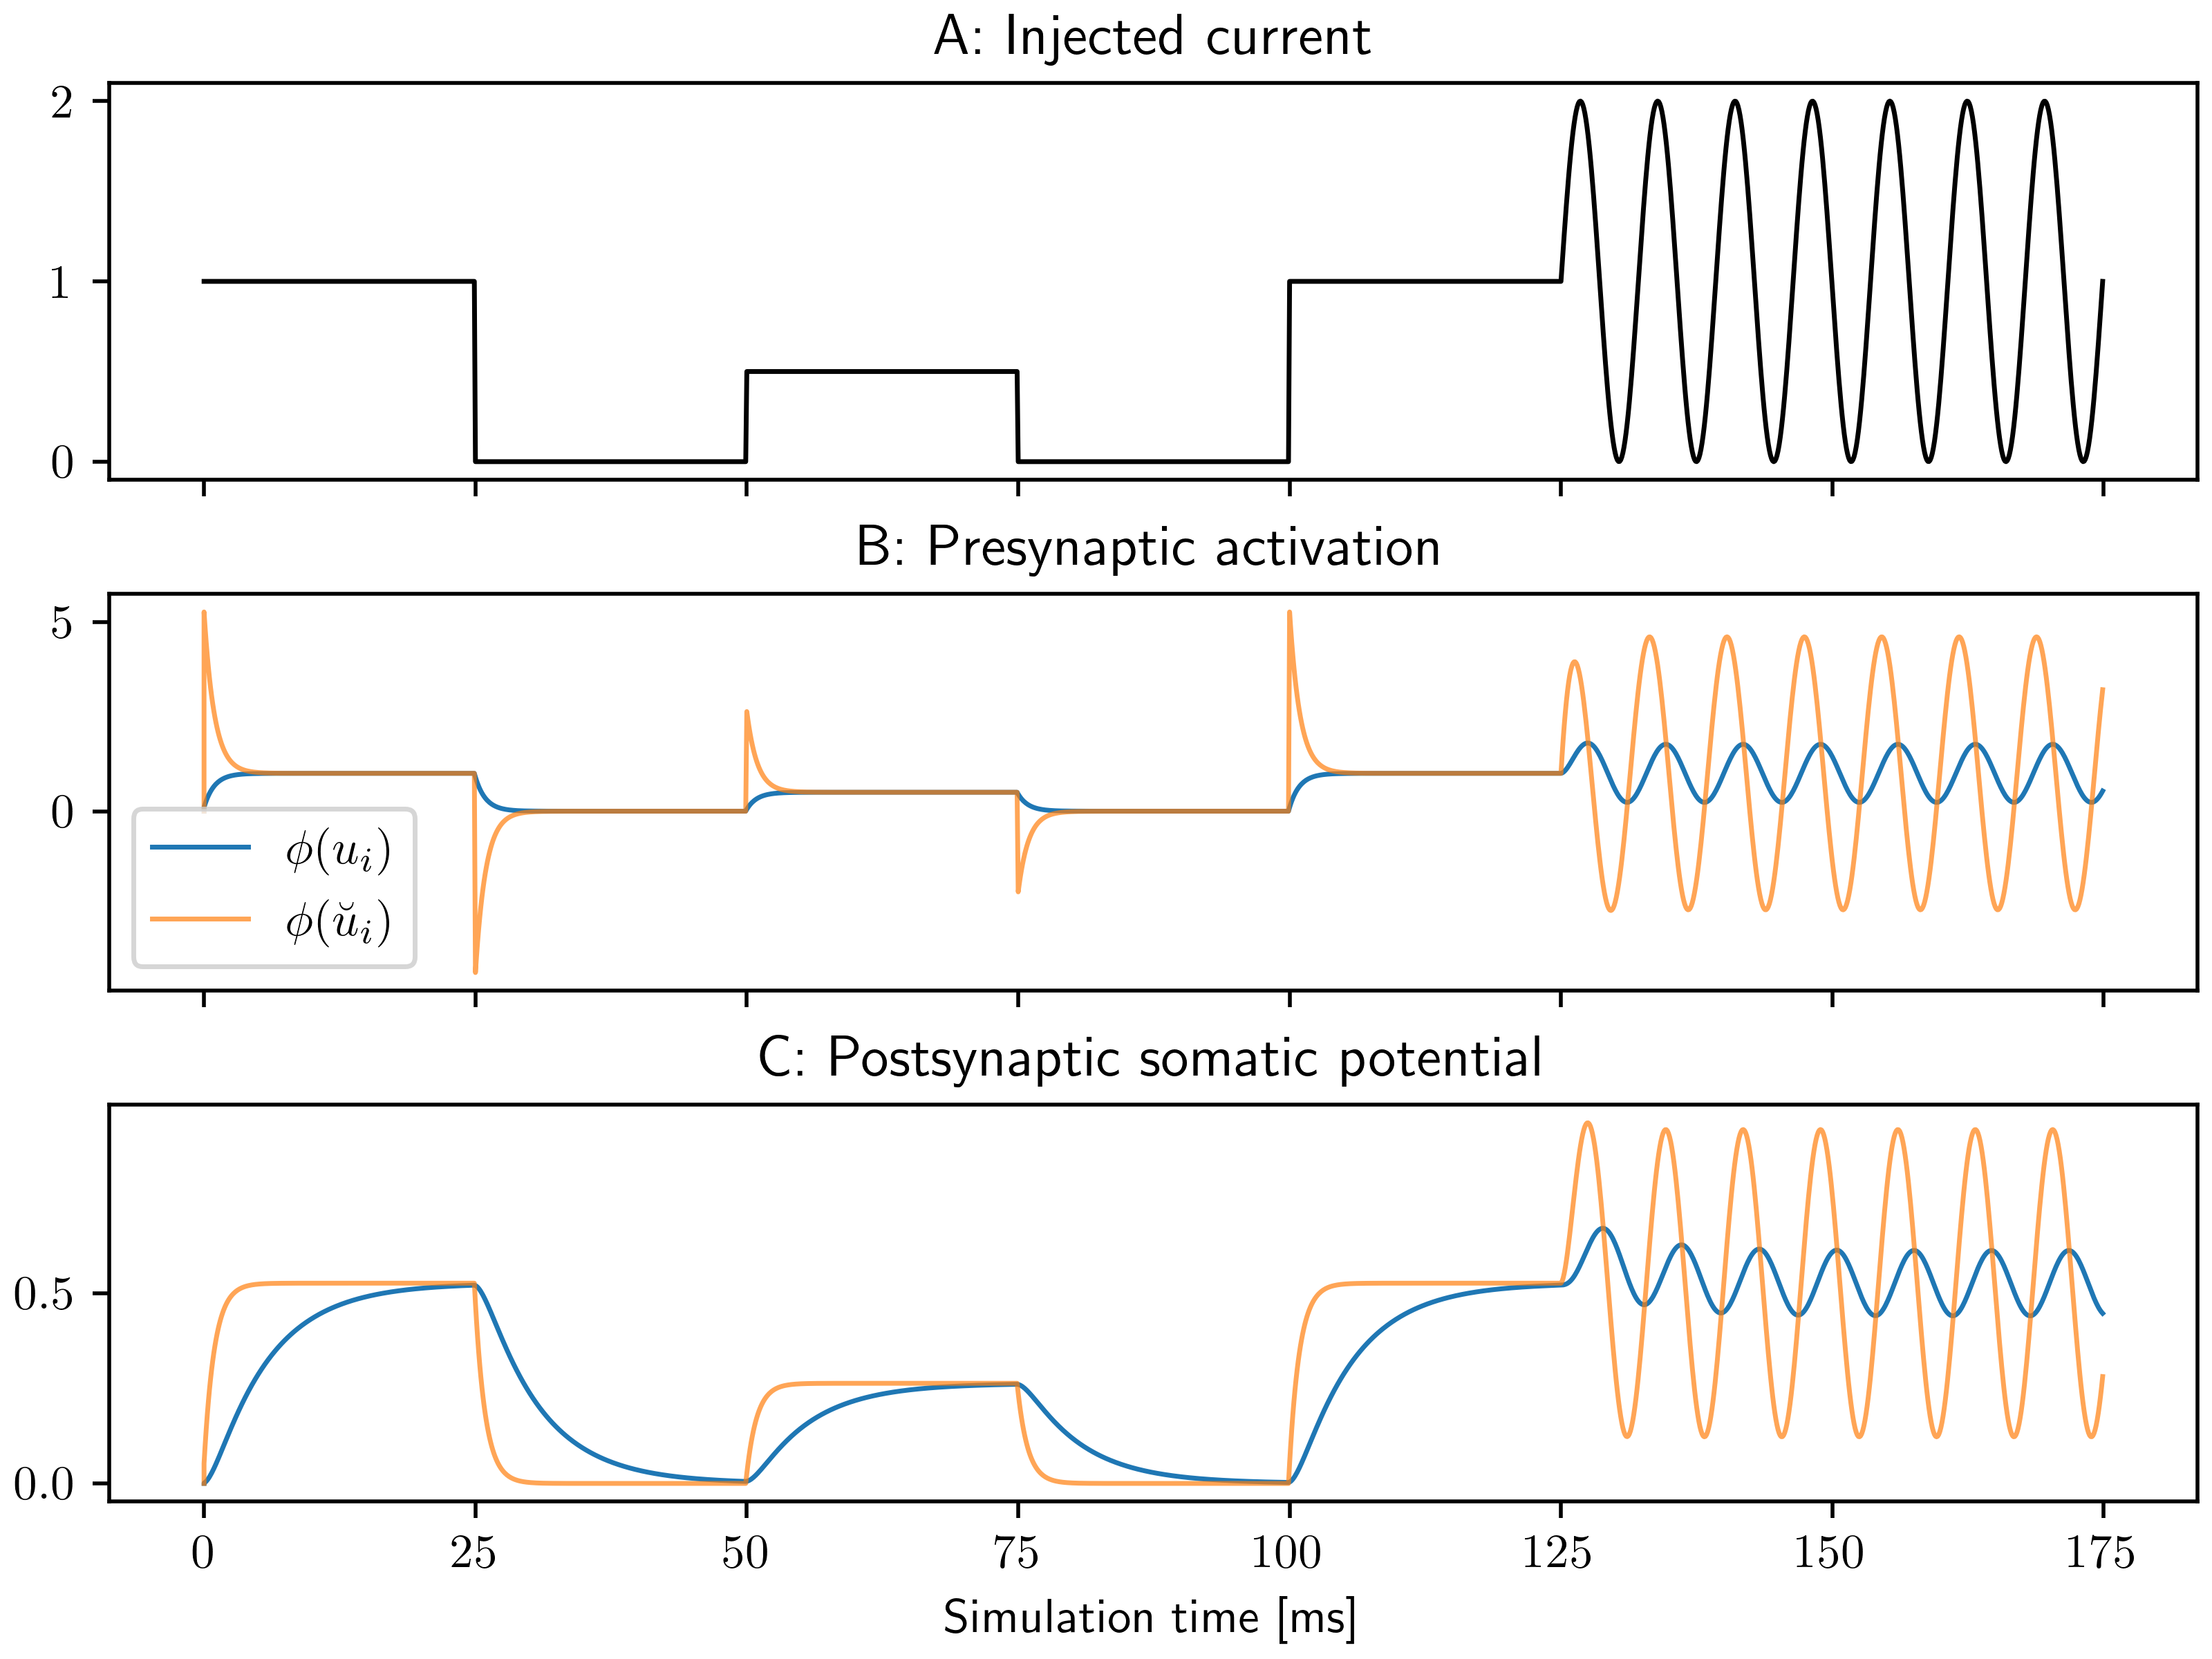
\includegraphics[width=0.9\textwidth]{fig_le_response}
  \caption[Signal transmission of LE neurons]{Signal transmission of LE neurons. Shown is a connection between an input
    neuron $i$ and a hidden layer pyramidal neuron $j$. Activations for the original Sacramento model (blue) and
    prospective activation using LE (orange) are compared. \textbf{A:} Current injected into the input neuron. Membrane
    potential slowly adapts to match this (not shown) \textbf{B:} Activation of the input neuron using instantaneous-
    $\phi(u_i)$ (blue), and prospective activation $\phi(\breve{u}_i)$ (orange). Note how strongly prospective
    activation reacts to changes in somatic voltage, leading to 'bursts' in neuron output. After the input neuron has
    reached its relaxed state ($\dot{u}_i = 0$), both mechanisms evoke the same activation. \textbf{C:} Somatic
    potential $u_j$ of the pyramidal neuron responding to signals sent from the input neuron (color scheme as in B).}
  \label{fig-comparison-le}
\end{figure}

When employing the default parametrization given by Haider et al. (Table \ref{tab-params}), $\tau_{eff}$ is slightly
lower than reported pyramidal neuron time constants \citep{McCormick1985} at approximately $5.26ms$. When presynaptic
neurons employ prospective dynamics, postsynaptic neurons approach their steady state much more quickly, as depicted in
Fig. \ref{fig-comparison-le}. In intuitive terms, prospective activation is more strongly dependent on the derivative
membrane potential compared to the instantaneous activation. This results in drastic changes in activation in response
to changes in the somatic membrane potential. While this can lead to an overshoot of postsynaptic activity, under
careful parametrization it strongly decreases response time.


\begin{figure}[h!]
  \centering
  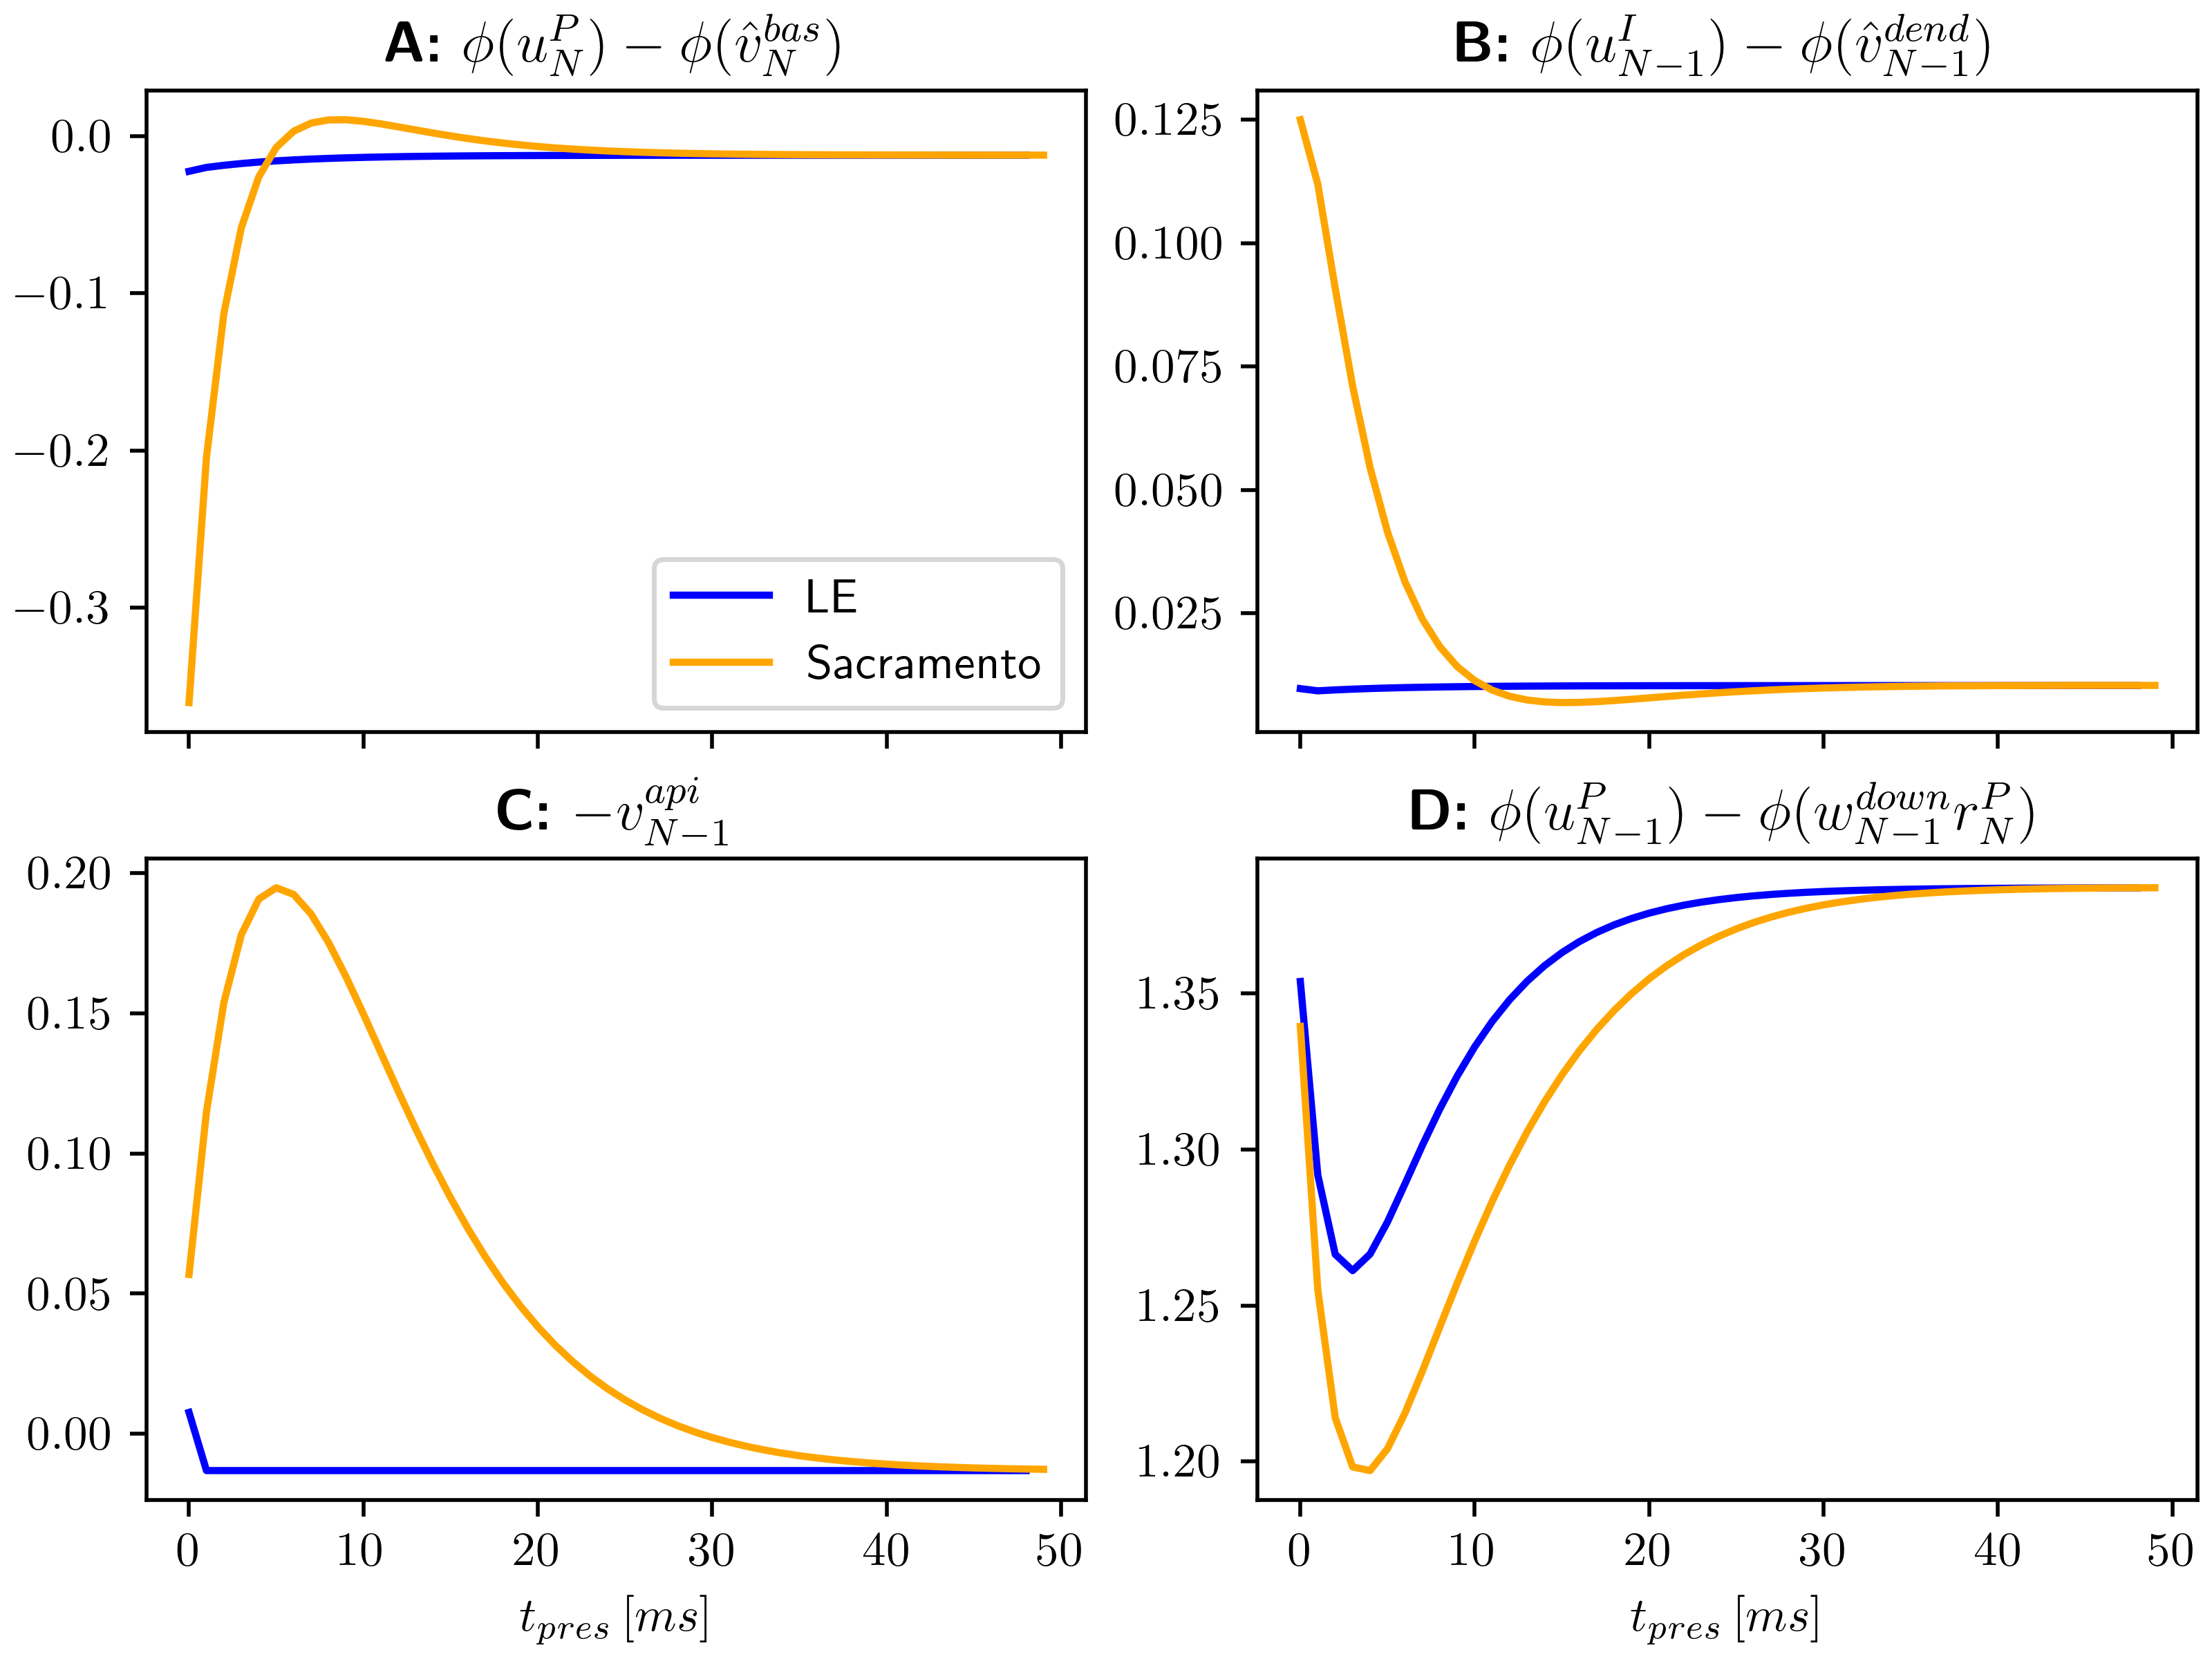
\includegraphics[width=0.9\textwidth]{fig_le_dendritic_errors}
  \caption[Effects of LE dynamics on dendritic error]{Effects of LE dynamics on the dendritic error terms from Equations
    \ref{eq-delta_w_up}-\ref{eq-delta_w_down}. Depicted are error terms for individual spiking neurons in a network with
    one hidden layer (N=3). The network was fully trained on the Bars dataset (cf. Section \ref{sec-le-tpres}), so
    errors should ideally relax to zero. Note, that this does not happen here due to the fluctuations inherent to the
    spiking network variant which was employed. In the original dendritic error network (orange), dendritic errors
    exhibit longer and more intense deviations, while errors in an identical LE network (blue) relax much sooner.
    \textbf{A:} Basal dendritic error for a pyramidal neuron at the output layer. \textbf{B:} Dendritic error for a
    hidden layer Interneuron. \textbf{C:} Proximal apical error for a hidden layer Pyramidal neuron. \textbf{D:} Distal
    apical error for the same pyramidal neuron. Note that this error term does not converge to zero for either network,
    an issue that will be discussed in Section \ref{sec-feedback-plast}.}
  \label{fig-error-comp-le}
\end{figure}


When employing prospective dynamics in the dendritic error networks, local error terms of pyramidal- and interneurons
relax much faster, as shown in Fig. \ref{fig-error-comp-le}. These simulations highlight the superiority of LE for
learning in this network, as the relaxation period is almost instantaneous. In contrast, the error terms in the original
dendritic error network drive random synaptic plasticity even when the network is fully trained on a given dataset and
is able to make accurate predictions. Thus, both the issue of redundant weight changes, as well as concerns over
response time and learning speed can be solved by LE. The authors furthermore show, that learning with this mechanism is
indifferent to presentation times or effective time constant for rate neurons. In addition to using the prospective
somatic potential for the neuronal transfer function, it is also used in the plasticity rule of LE neurons. The
Urbanczik-Senn plasticity is therefore updated to compute dendritic error from prospective somatic activations and a
non-prospective dendritic potential $\dot{w}_{ij}= \eta \ ( \phi(\breve{u}_i^{som}) - \phi(\hat{v}_i^{bas}) ) \
  \phi(\breve{u}_j^{som})^T$. Much like for the transfer function, this change serves to increase the responsiveness of
the network to input changes.

\section{Implementational details}

Building on the neuron and plasticity model from \citep{Stapmanns2021}, a replicate model of the pyramidal neuron with
spike-based communication was developed in NEST. The existing neuron model was expanded to three compartments, and
storage and readout of dendritic errors were updated  to allow for compartment-specific plasticity rules. Interneurons
were chosen to be modeled as pyramidal neurons with slightly updated parameters and apical conductance $g^{api}=0$.
Since membrane dynamics of both neurons follow the same principles and additional compartments have minor impact on
performance, this was deemed sufficient.

After facing some setbacks when attempting to train the first spiking variant of the network, the decision was made to
also implement a rate-based variant of the neuron in NEST.  While the additional effort required for another
implementation might be questionable, this model turned out to be indispensible. It enabled the identification of both
errors in the model, as well as training mechanisms and parameters that required changes to enable spike-compatible
learning. The rate version in NEST additionally served to distinguish discrepancies that are due to the novel simulation
backend from those that were introduced by the spike-based communication scheme.

Following NEST convention, the spiking and rate-based neuron models were named \texttt{pp\_\allowbreak cond\_\allowbreak
  exp\_\allowbreak mc\_\allowbreak pyr}\footnote{Despite being somewhat cryptic, the name does actually make sense, as
  it describes some key features of the model: It is a \textbf{point process} for \textbf{cond}uctance based synapses
  and has an \textbf{exp}onentially decaying membrane in \textbf{multiple compartments}.} and \texttt{rate\_\allowbreak
  neuron\_\allowbreak pyr} respectively. Furthermore, the \texttt{pyr\_\allowbreak synapse} class was defined for spike
events, and implements the event-based variant of the Urbanczik-Senn plasticity described in Section
\ref{sec-event-urb}. The \texttt{pyr\_\allowbreak synapse\_\allowbreak rate} model on the other hand transmits rate
events and updates its weight according to the original plasticity rule.

Simulations were managed using the python API \texttt{PyNEST} \citep{Eppler2009}, which is much more convenient than the
SLI interface that lies at the core of NEST. An additional advantage of using this language is, that the LE network  is
also implemented in python. Thus, by including a slightly modified version of that code in my project, it was possible
to unify all three variants in a single network class and accompanying interface. This allowed for exact alignment of
network stimulation and readout and enabled in-depth comparative analyses. In some of the upcoming Results, three
variants of the same network architecture will therefore be compared; The modified python implementation from
\citep{Haider2021} is termed \texttt{NumPy} based on the framework that is used to compute neuron dynamics and synaptic
plasticity through matrix multiplication. The two NEST variants will be referred to as \textit{NEST spiking} and
\textit{NEST rate}.

\subsection{Neuron model Adaptations}

The neuron model from \citep{Stapmanns2021} was modified in several ways in order to match the pyramidal neuron
implementation more closely. Both the inclusion of nonzero reversal potentials and the flow of currents from the soma to
the dendrites were omitted in my model. Furthermore, the present network requires synapses to be able change the sign of
their weight at runtime, which is not permitted in the original synapse model. For this reason, the strict separation of
excitatory and inhibitory synapses had to be removed from the synapse model. In order to compare the different
implementations exactly, the ODE solver with variable stepsize was replaced with Euler integrations\footnote{This change
  initially served debugging purposes, but turned out to have no negative effect on performance and was therefore kept.}
with step size $\Delta t$. For the spiking neuron model, dendritic compartments are modeled with leaky membrane dynamics
in contrast to the rate variant. The choice of dendritic leakage conductance $g_l^{dend}=\Delta t=0.1$ is motivated in
Section \ref{sec-gl-dend}.

A major issue of the spiking network is the fact that under the default parametrization, spikes are too infrequent for
the network to accurately compute the dendritic error terms. Initial experiments showed that the network is rather
sensitive to changes in parametrization, which meant that it was desirable to change as few existing parameters as
possible. Therefore, a novel parameter $\psi$ was introduced. In a spiking neuron $i$, the probability of eliciting a
spike is linearly increased by this factor ($r_i = \psi \phi(u_i)$). Likewise, all synaptic weights $W$ in a spiking
network are attenuated by the same factor ($W \leftarrow \frac{W}{\psi}$). These changes cancel each other out, as an
increased value for $\psi$ elicits no change in absolute compartment voltages of a network. Instead, it serves to
stabilize these voltages over time, which drastically improves learning performance. One mechanism in which this
parameter also needs to be considered is the plasticity rule. Weight changes are affected by $\psi$ in three distinct
ways: Since $\psi$ is linearly scales the activation (spiking or hypothetical), it also increases dendritic error
linearly, as it does the presynaptic activation. Additionally, since the frequency of weight changes is determined by
the presynaptic spike rate, $\psi$ increases the strength of plasticity three times. As these influences are
multiplicative, learning rates are attenuated by $\eta \leftarrow \frac{\eta}{\psi^3}$. The exception to this are the
weights from interneurons to pyramidal neurons, as these do not depend on dendritic predictions, but on absolute
dendritic voltage. Hence, in this case $\eta^{pi} \leftarrow\frac{\eta^{pi}}{\psi^2}$. On close investigation of the
spiking neuron model, one can observe that for $\psi \rightarrow \infty$, it approximates the rate-based implementation
exactly at the steady state. Unsurprisingly therefore, increasing $\psi$ caused the spiking network to learn
successfully with fewer samples and to a lower test loss. Yet, the argument against increasing $\psi$ is twofold:
Initial experiments showed that only for $\psi < 0.1$ did pyramidal and interneurons exhibit spike frequencies in
biologically plausible range of less than $55Hz$ \citep{Kawaguchi2001,Eyal2018}. Additionally, each transmitted
\texttt{SpikeEvent} is computationally costly, which increases training time (cf. Fig. \ref{fig-benchmark-threads-psi})
and therefore further makes high spike frequencies undesirable. As a middle ground, $\psi = 100$ proved useful during
initial tests and will be assumed the default from here on out. Note that this parametrization was chosen primarily with
efficiency in mind, and is far removed from biologically plausible spike frequencies. With these adaptations, the
network was able to perform supervised learning with spiking neurons, as will be discussed in the upcoming sections.

\section{Error metrics and nomenclature}

In this thesis, the word 'error' is used frequently, which might understandably lead to confusion. While stylistically
questionable, this choice was made deliberately to conform to the main underlying works
\citep{urbanczik2014learning,sacramento2018dendritic,whittington2019theories,Haider2021}. This section will provide a
brief disambiguation. Firstly, there are four error metrics describing the network's deviation from the self-predicting
state: \textit{Feedforward weight error (FF error), Feedback weight error (FB error), Apical error and Interneuron
  error}. These were introduced in Section \ref{sec-selfpred}\footnote{Observation of the network dynamics reveals that
  pairs of them are closely related: FF error drives interneuron error, and FB error drives apical error as soon as
  interneuron error is minimal. An analytical upgrade to this model might include a way for unifying these pairs of
  metrics.}. Furthermore, three terms require elaboration:\newline

\textbf{Dendritic error}: Any value which drives the Dendritic plasticity rules. Classically, this refers to a failure
of a dendrite to predict somatic activity \citep{urbanczik2014learning}. In this context, due to the changes to the
plasticity rule, it may also refer to absolute voltage of pyramidal neuron apical compartments (i.e. Apical error).
\newline

\textbf{Train error}: Failure rate of a network to correctly classify inputs during testing. In the upcoming
simulations, all targets are encoded with one-hot vectors. Thus, accuracy is defined as:
\begin{align*}
  accuracy & = \frac{1}{N} \sum_{i=1}^N \  \delta \left(argmax(y^{target}_i),\ argmax(y^{pred}_i) \right)
\end{align*}
for a test run over $N$ samples, with $\delta$ being the Kronecker delta function. Train error is defined as inverse
accuracy.\newline

\textbf{Loss}: Unless specified otherwise, train- and test loss are are computed through MSE between predicted and
target output:
\begin{align*}
  MSE & = \frac{1}{M} \sum_{i=1}^M \left( y^{target}_i-y^{pred}_i \right)^2
\end{align*}
With $M$ neurons in the output layer, which is again averaged over $N$ test samples. Due to the network's relaxation
period, $y^{pred}$ can not be accurately computed instantaneously\footnote{Sacramento et al. actually do exactly this.
  They compute $y^{pred}$ without neuron dynamics, only from the input, activation function $\phi$, and feedforward
  weights. This approach makes the assumption that the network is permanently in a perfect self-predicting state, in
  which lateral and feedback weights have no impact on pyramidal neuron activity. Particularly for the spiking variant,
  this assumption was shown to be erroneous, leading to artificially inflated performance. Hence, all tests are
  performed by fully simulating networks with disabled plasticity.}. Instead, the network needs to be presented with the
stimulus for a given time $t_{pres}$. Particularly for the SNN, as well as networks injected with noise, output layer
membranes fluctuate strongly. therefore, $y^{pred}$ is an average over recorded somatic potentials for each output
neuron. This recording typically starts after $\sim 70\%$ of $t_{pres}$ has passed.